%%%%%%%%%%%%%%%%%%%%%%%%%%%%%%%%%%%%%%%%%
% Short Sectioned Assignment LaTeX Template Version 1.0 (5/5/12)
% This template has been downloaded from: http://www.LaTeXTemplates.com
% Original author:  Frits Wenneker (http://www.howtotex.com)
% License: CC BY-NC-SA 3.0 (http://creativecommons.org/licenses/by-nc-sa/3.0/)
%%%%%%%%%%%%%%%%%%%%%%%%%%%%%%%%%%%%%%%%%

%----------------------------------------------------------------------------------------
%	PACKAGES AND OTHER DOCUMENT CONFIGURATIONS
%----------------------------------------------------------------------------------------

\documentclass[paper=a4, fontsize=11pt]{scrartcl} % A4 paper and 11pt font size

% ---- Entrada y salida de texto -----

\usepackage[T1]{fontenc} % Use 8-bit encoding that has 256 glyphs
\usepackage[utf8]{inputenc}
%\usepackage{fourier} % Use the Adobe Utopia font for the document - comment this line to return to the LaTeX default

% ---- Idioma --------

\usepackage[spanish, es-tabla]{babel} % Selecciona el español para palabras introducidas automáticamente, p.ej. "septiembre" en la fecha y especifica que se use la palabra Tabla en vez de Cuadro

% ---- Otros paquetes ----

\usepackage{url} % ,href} %para incluir URLs e hipervínculos dentro del texto (aunque hay que instalar href)
\usepackage{amsmath,amsfonts,amsthm} % Math packages
%\usepackage{graphics,graphicx, floatrow} %para incluir imágenes y notas en las imágenes
\usepackage{graphics,graphicx, float} %para incluir imágenes y colocarlas
\usepackage{epstopdf}

% Para hacer tablas comlejas
%\usepackage{multirow}
%\usepackage{threeparttable}

%\usepackage{sectsty} % Allows customizing section commands
%\allsectionsfont{\centering \normalfont\scshape} % Make all sections centered, the default font and small caps

\usepackage{fancyhdr} % Custom headers and footers
\pagestyle{fancyplain} % Makes all pages in the document conform to the custom headers and footers
\fancyhead{} % No page header - if you want one, create it in the same way as the footers below
\fancyfoot[L]{} % Empty left footer
\fancyfoot[C]{} % Empty center footer
\fancyfoot[R]{\thepage} % Page numbering for right footer
\renewcommand{\headrulewidth}{0pt} % Remove header underlines
\renewcommand{\footrulewidth}{0pt} % Remove footer underlines
\setlength{\headheight}{13.6pt} % Customize the height of the header

\numberwithin{equation}{section} % Number equations within sections (i.e. 1.1, 1.2, 2.1, 2.2 instead of 1, 2, 3, 4)
\numberwithin{figure}{section} % Number figures within sections (i.e. 1.1, 1.2, 2.1, 2.2 instead of 1, 2, 3, 4)
\numberwithin{table}{section} % Number tables within sections (i.e. 1.1, 1.2, 2.1, 2.2 instead of 1, 2, 3, 4)

\setlength\parindent{0pt} % Removes all indentation from paragraphs - comment this line for an assignment with lots of text

\newcommand{\horrule}[1]{\rule{\linewidth}{#1}} % Create horizontal rule command with 1 argument of height


%----------------------------------------------------------------------------------------
%	TÍTULO Y DATOS DEL ALUMNO
%----------------------------------------------------------------------------------------

\title{	
\normalfont \normalsize 
\textsc{\textbf{Curso 2016-2017} \\ Grado en Ingeniería Informática \\ Universidad de Granada} \\ [25pt] % Your university, school and/or department name(s)
\horrule{0.5pt} \\[0.4cm] % Thin top horizontal rule
\huge Cuestionario 3 \\ % The assignment title
\horrule{2pt} \\[0.5cm] % Thick bottom horizontal rule
}

\author{Carlos Manuel Sequí Sánchez} % Nombre y apellidos

\date{\normalsize\today} % Incluye la fecha actual

%----------------------------------------------------------------------------------------
% DOCUMENTO
%----------------------------------------------------------------------------------------

\begin{document}

\maketitle % Muestra el Título

\newpage %inserta un salto de página

\newpage



\begin{figure}[H]
	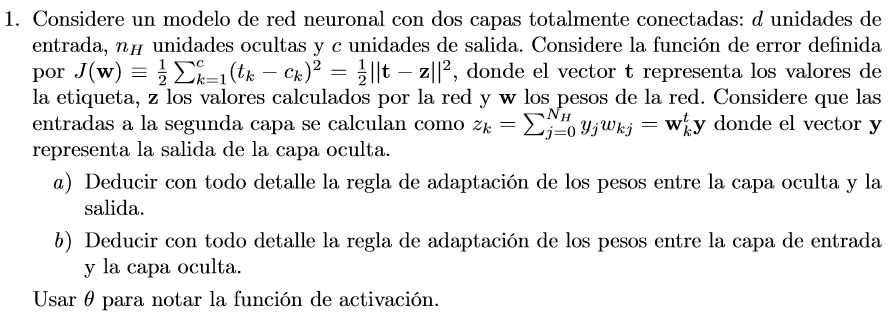
\includegraphics[scale=0.65]{imagenes/1} 
\end{figure}

\newpage

\begin{figure}[H]
	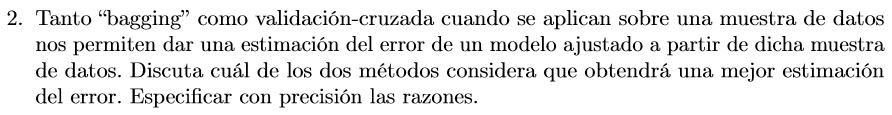
\includegraphics[scale=0.65]{imagenes/2} 
\end{figure}

Fuente: Transparencias de teoría de la asignatura de Aprendizaje Automático (UGR).

La técnica del \textbf{Bagging} es una mezcla entre la técnica de Bootstrap y promedios:
\begin{itemize}
	\item \textbf{Bootstrap:} consiste en realizar X conjuntos de datos de entrenamiento del mismo tamaño que el conjunto original, remuestreando de forma aleatoria y con reemplazamiento para obtener nuevas muestras, dando así la posibilidad de tener elementos repetidos dentro del conjunto Xi y, por tanto, pudiendo dejar muestras fuera de dicho subconjunto. Una vez obtenidos los dataset con los que vamos a entrenar nuestros modelos (conjunto de datos Train), obtenemos los conjuntos de datos de validación (los datos para el Test), los cuales serán todas aquellas muestras que no hayan sido escogidas en los subconjuntos del Train(por lo general 1/3 de los datos del conjunto inicial de datos son usados para el conjunto de datos Test). Uno de los problemas de esta técnica es que los árboles de decisión creados presentan una alta varianza y, es por ello por lo que usamos Bagging, para reducir esa gran varianza.
	
	\item \textbf{Promedios:} Con el fin expuesto, Bagging construye X árboles de regresión usando los X conjuntos de entrenamiento generados por Bootstrap y realiza el promedio de las predicciones resultantes. Al realizar dicho promedio (teniendo en cuenta que los árboles inicialmente no están podados) la varianza se reduce considerablemente, obteniendo una técnica con un cierto nivel en la relación sesgo-varianza.
\end{itemize}


La técnica de \textbf{validación cruzada} consiste en hacer X pares de conjuntos Train-Test de manera que utilicemos a la hora de validar una medida del error promedio con las sucesivas particiones creadas y obtener así una validación más fiable y ajustada que realizándola únicamente sobre un solo conjunto de datos. Los subconjuntos Train y Test creados en el caso de la validación cruzada son disjuntos, por lo que no tenemos datos repetidos entre ambos subconjuntos. Además cada par Train-Test de los X pares creados para la validación del modelo son distintos, de esta forma en cada par de conjuntos Test-Train creado tenemos que los subconjuntos Test son completamente distintos entre ellos, haciendo que la validación se realice cada vez con un subconjunto del dataset distinto, lo cual hace que el ajuste del error sea alto.\\
Para calcular el error simplemente se obtiene todos los $Eout_i$ correspondientes a cada par de particiones Test-Train y se calcula la media de dichos errores, lo que nos dará el $E_{cv}$ \\

Como conclusión sobre la mejor de las estimaciones obtenidas comparando Cross Validation(CV) con Bagging, pienso que el hecho de que CV utilice todos y cada uno de los datos para aprender mediante distintos conjuntos Train en las sucesivas particiones, es un hecho relevante a la hora de estimar el mejor modelo para ajustarnos a la función buscada, cosa que Bagging no hace, ya que este último ofrece completa libertad para que en el conjunto de Train haya muestras repetidas, lo que produce que no se aprenda con todos y cada una de las muestras del dataset como hace CV. Debido también a este motivo explicado, Bagging consta con un mayor poder de generalización, ya que ajusta menos el predictor a los datos del Train sin embargo, ni Bagging ni CV sufren los efectos del sobreajuste, por lo que no es un motivo para decantarse por una u otra técnica.\\
Bagging aumenta el ratio de predicción al tener varios árboles en contraste con un solo árbol.\\
En definitiva, y como última diferencia, pienso que no conviene utilizar Bagging frente a CV por el hecho de que, aun siendo un poco mejor a la hora de la predicción, la interpretación de los resultados es muy complicada, por tanto, teniendo en cuenta todo lo comentado hasta el momento pienso que la mejor estimación del error la hará la técnica de Validación Cruzada.


\begin{figure}[H]
	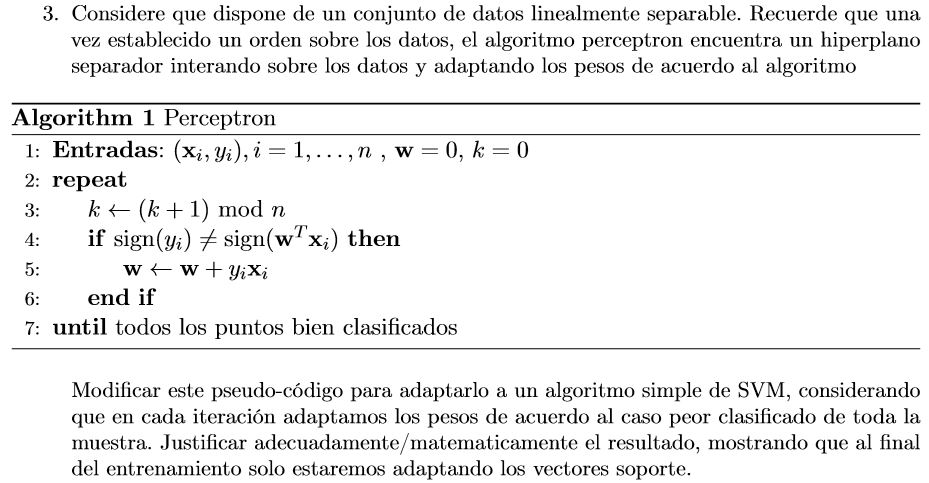
\includegraphics[scale=0.65]{imagenes/3} 
\end{figure}

\begin{figure}[H]
	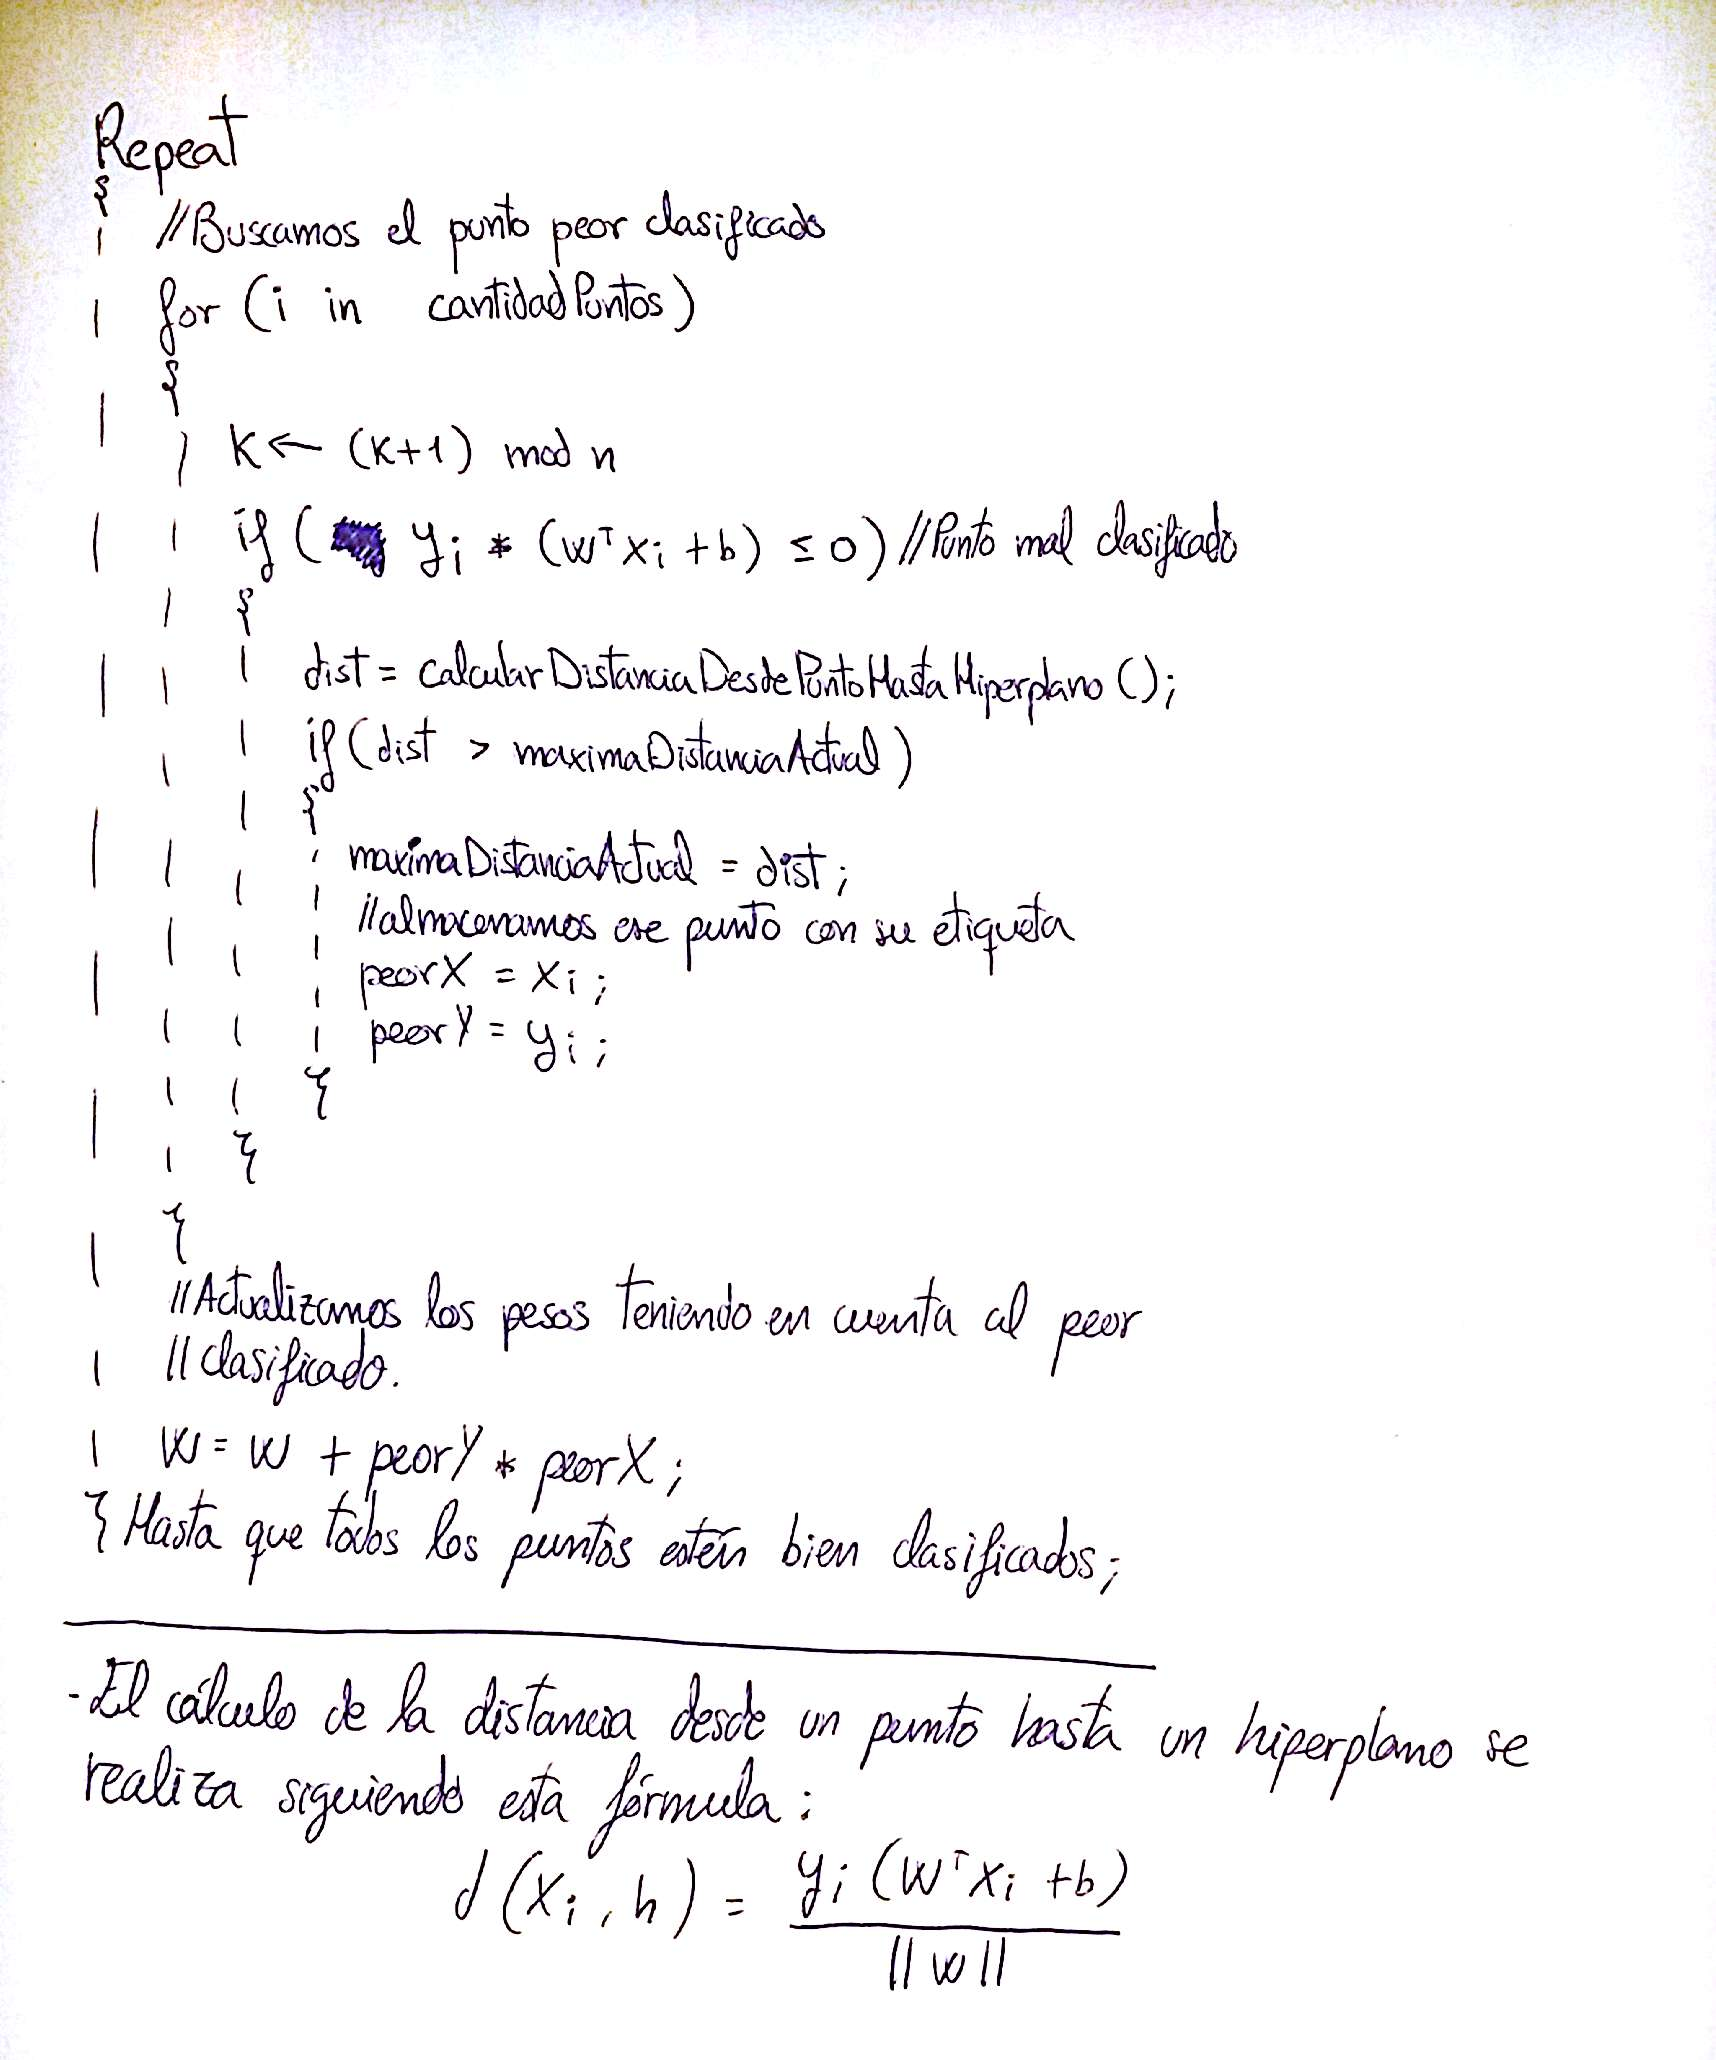
\includegraphics[scale=0.30]{imagenes/ej3} 
\end{figure}

\newpage

\begin{figure}[H]
	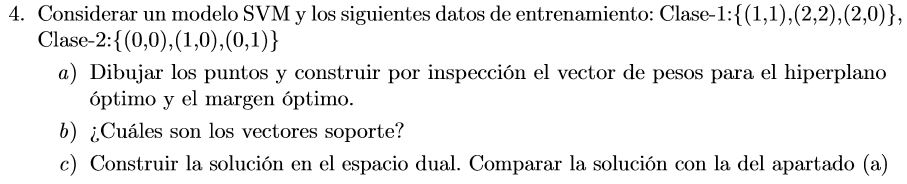
\includegraphics[scale=0.65]{imagenes/4} 
\end{figure}


\begin{figure}[H]
	\centering
	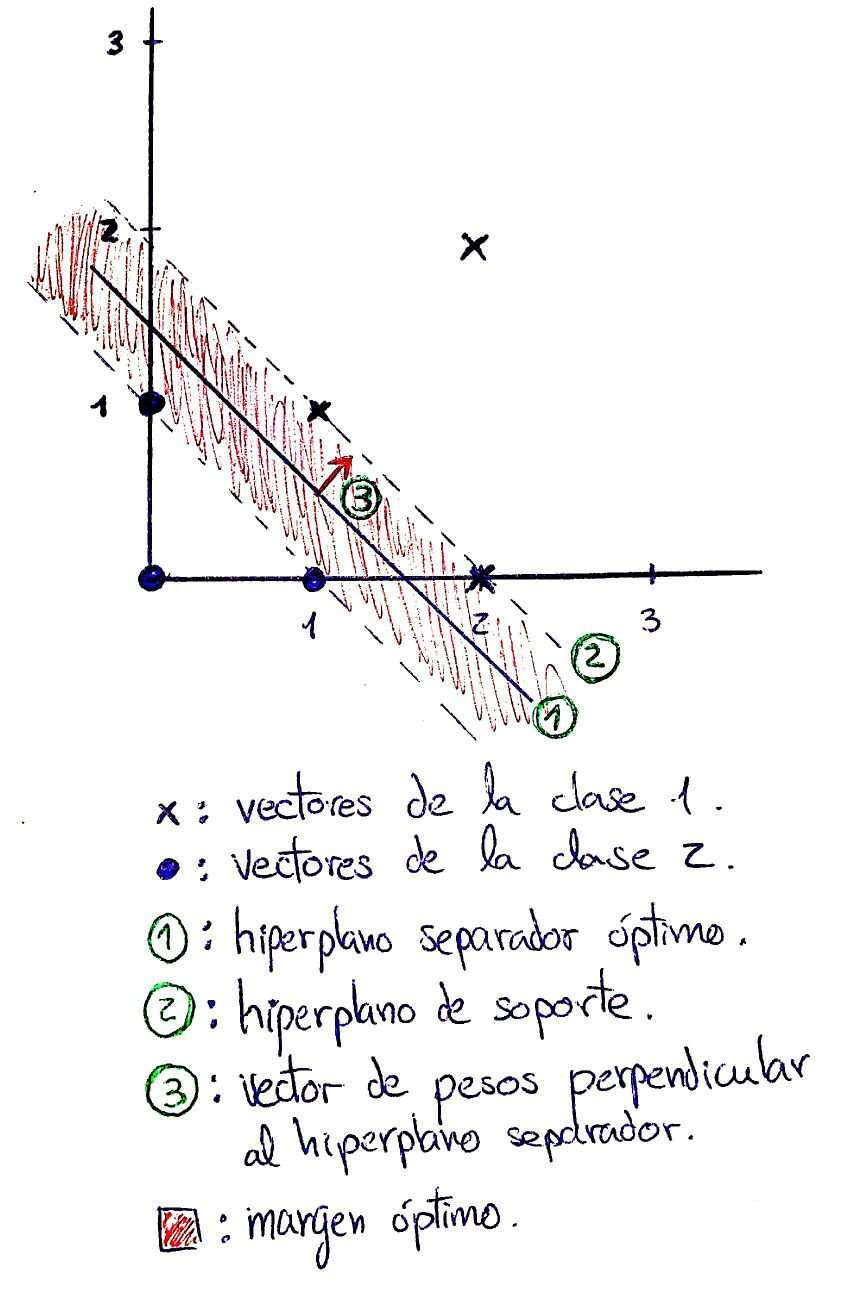
\includegraphics[scale=0.35]{imagenes/ej4} 
	\caption{\textbf{Apartado A}} \label{etiq}
\end{figure}

\textbf{APARTADO B:}\\
Vectores de soporte:
\begin{itemize}
	\item \textbf{Clase 1:} \{(1,0),(0,1)\}
	\item \textbf{Clase 2:} \{(2,0),(1,1)\}
\end{itemize}

\textbf{APARTADO C:}\\

\newpage

\begin{figure}[H]
	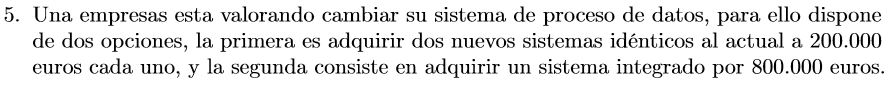
\includegraphics[scale=0.65]{imagenes/51} 
	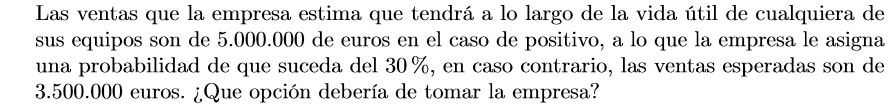
\includegraphics[scale=0.65]{imagenes/52} 
\end{figure}

Debido a la ambigüedad del enunciado, procedo a dar mis dos propias interpretaciones sobre el mismo.

\textbf{Interpretación del enunciado 1}
Considero que los dos sistemas que cuestan 200.000 euros cada uno son independientes, por lo que cada uno de ellos puede llegar a generar 5.000.000 de euros en caso de funcionar con el máximo rendimiento. El sistema integrado, tal y como dice el enunciado, también puede llegar a generar 5.000.000 de euros en el caso positivo.

Una vez realizada la interpretación es trivial llegar a la conclusión óptima para las ganancias de la empresa:

\begin{itemize}
	\item Por un lado tenemos que las dos máquinas idénticas a la actual pueden llegar a generar a la empresa un beneficio máximo de 10.000.000 de euros en caso de que ambas tengan una máxima productividad. En el caso opuesto, nos encontramos con que ambas máquinas trabajan a mínimo rendimiento y generan cada una 3.500.000 euros (7.000.000 euros en total).
	\item En el caso del sistema integrado tenemos que a máximo rendimiento, tal como expresa el enunciado puede generar 5.000.000 euros, mientras que a mínimo rendimiento puede generar 3.500.000 euros.
\end{itemize}

A la vista de la información expuesta, está claro que es preferible comprar dos máquinas por 400.000 euros para obtener una ganancia mayor (en cualquiera de los casos) que comprando una sola máquina por 800.000 euros con la cual es posible que la empresa no gane ni la mitad que con los dos sistemas.\\
Reiterando un poco lo afirmado, cabe destacar que en caso de comprar las dos máquinas y que trabajen a mínimo rendimiento la empresa obtendría más ganancias (7 millones de euros) que si comprase sel sistema integrado y éste trabajase a máximo rendimiento (5 millones de euros).\\

\textbf{Interpretación del enunciado 2:}\\
En la siguiente página muestro la resolución del ejercicio con la segunda interpretación, en la cual considero que los dos sistemas pueden obtener de forma conjunta una ganandia de 5.000.000 euros (en lugar de 10.000.000) y que si una sola falla, entonces la ganancia es de 3.500.000 euros.

\newpage

\begin{figure}[H]
	\centering
	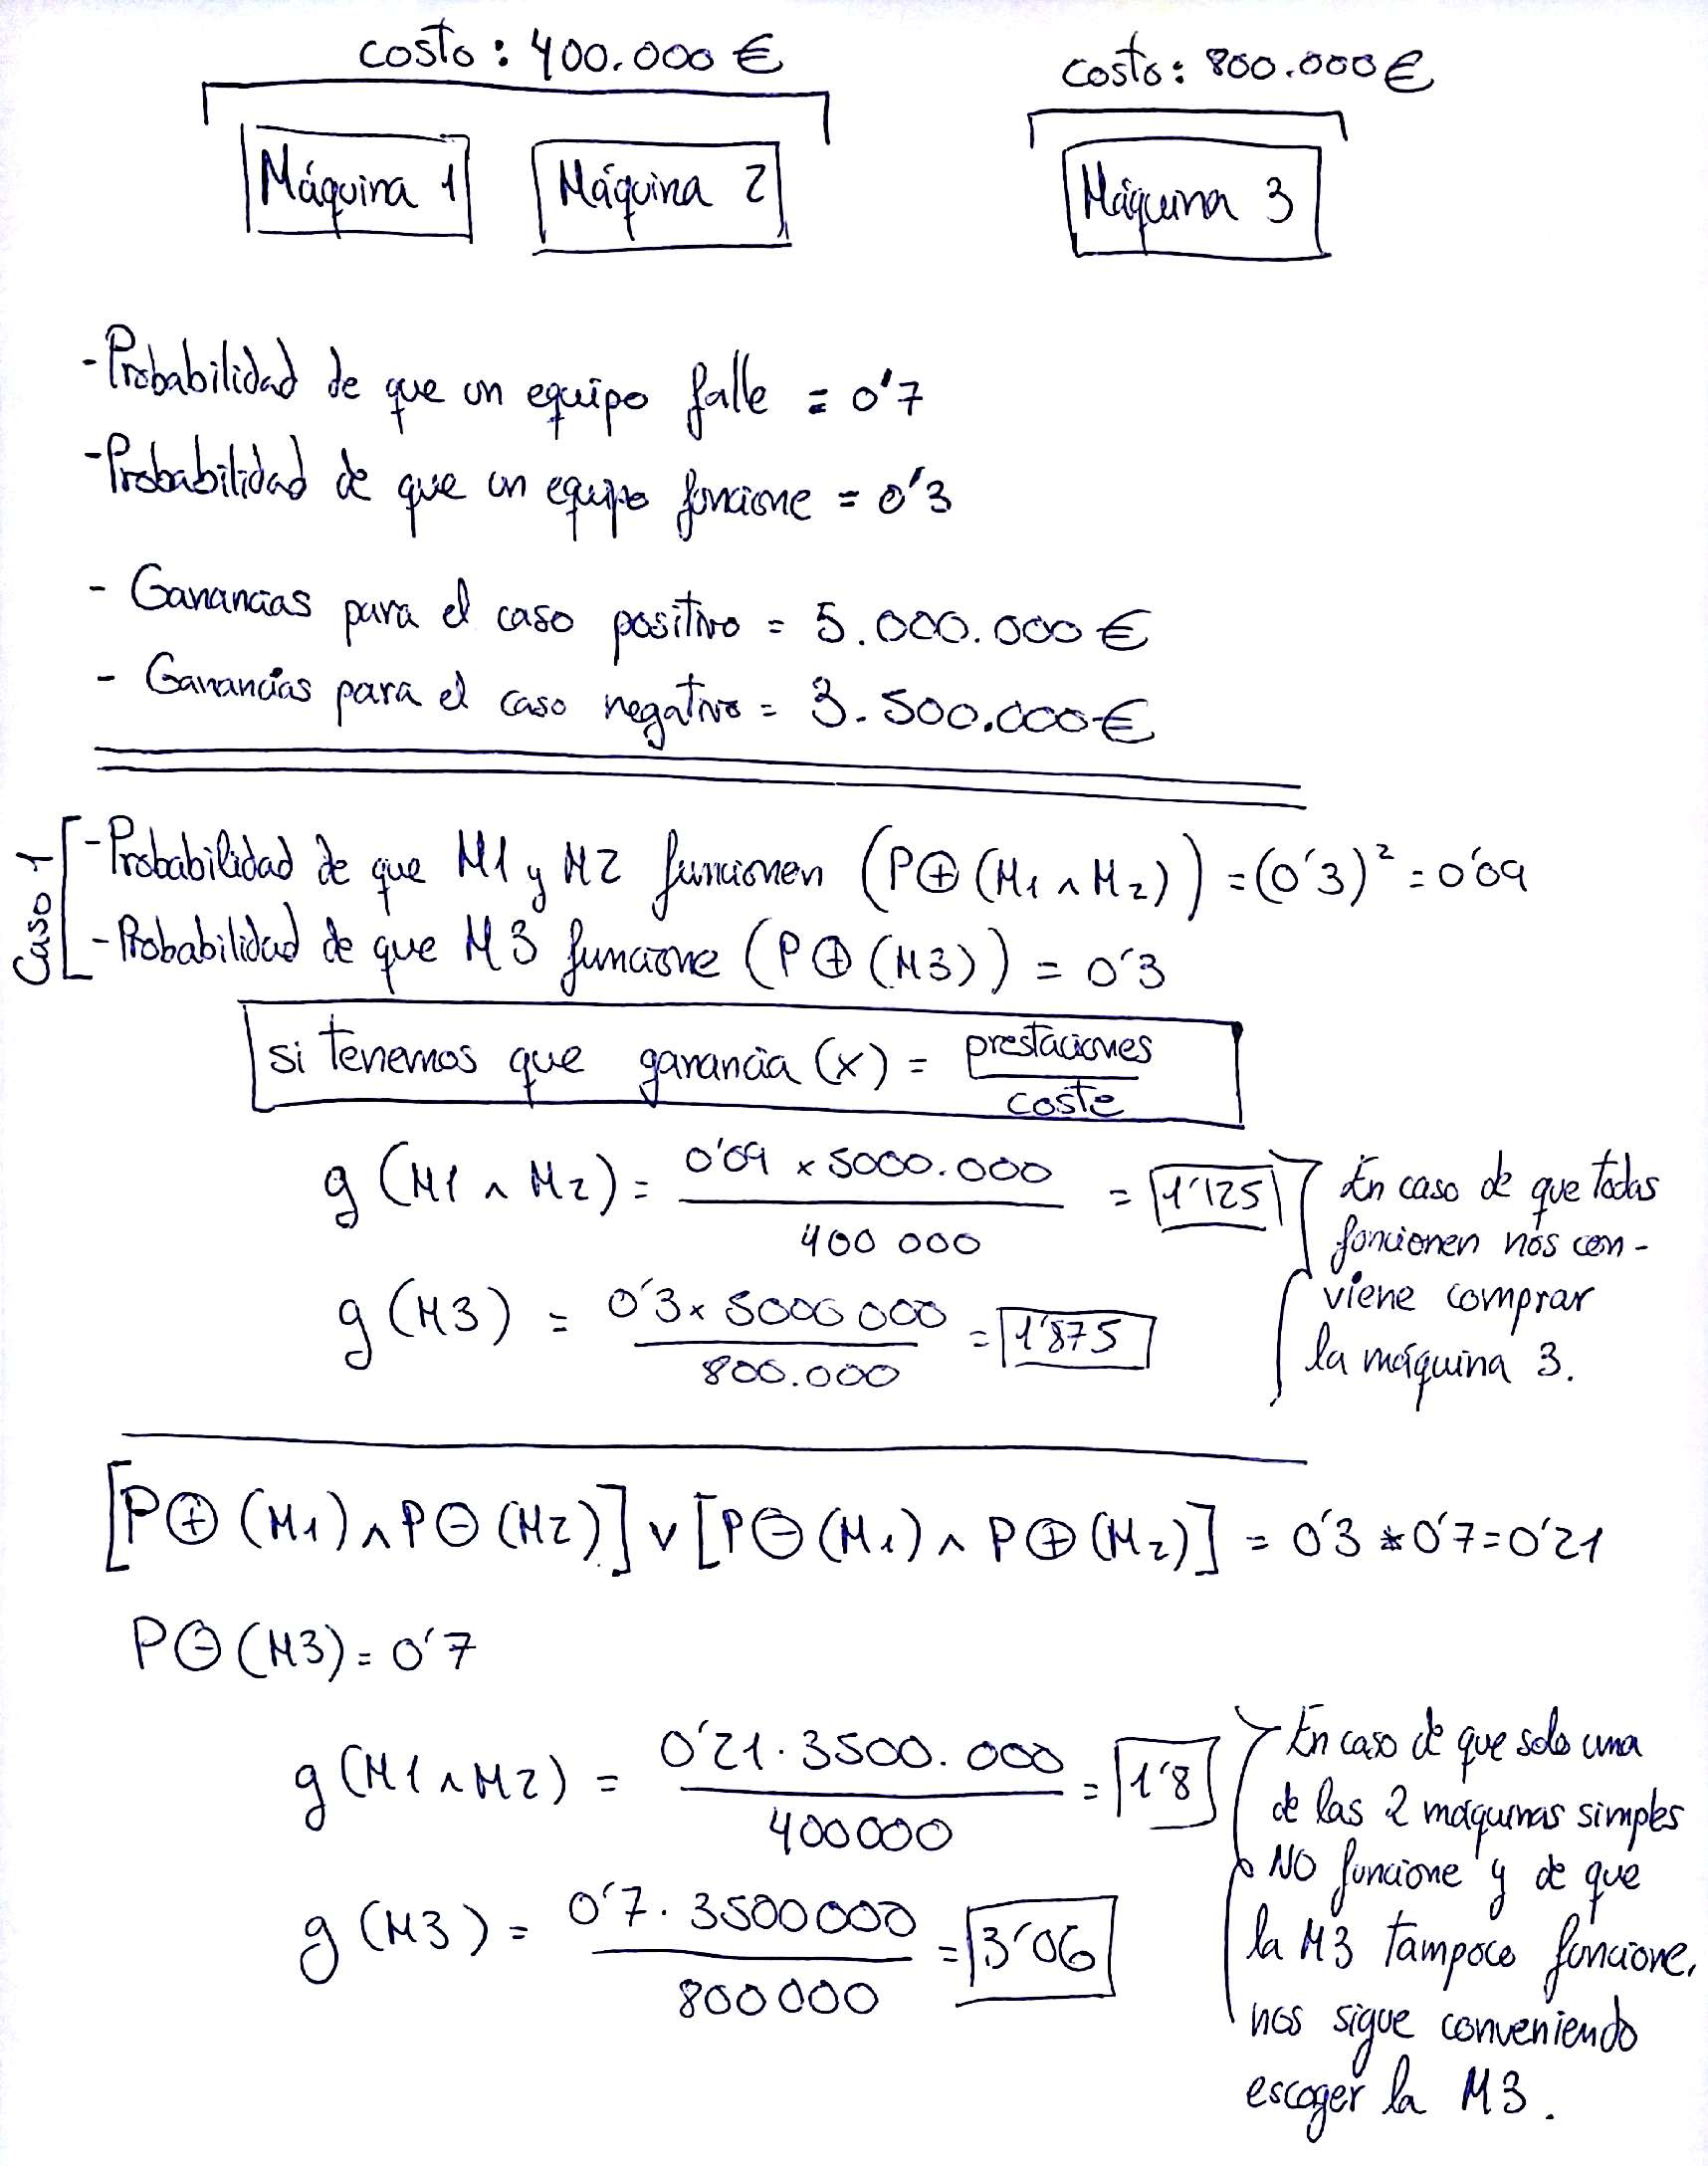
\includegraphics[scale=0.28]{imagenes/ej51} 
\end{figure}

\begin{figure}[H]
	\centering
	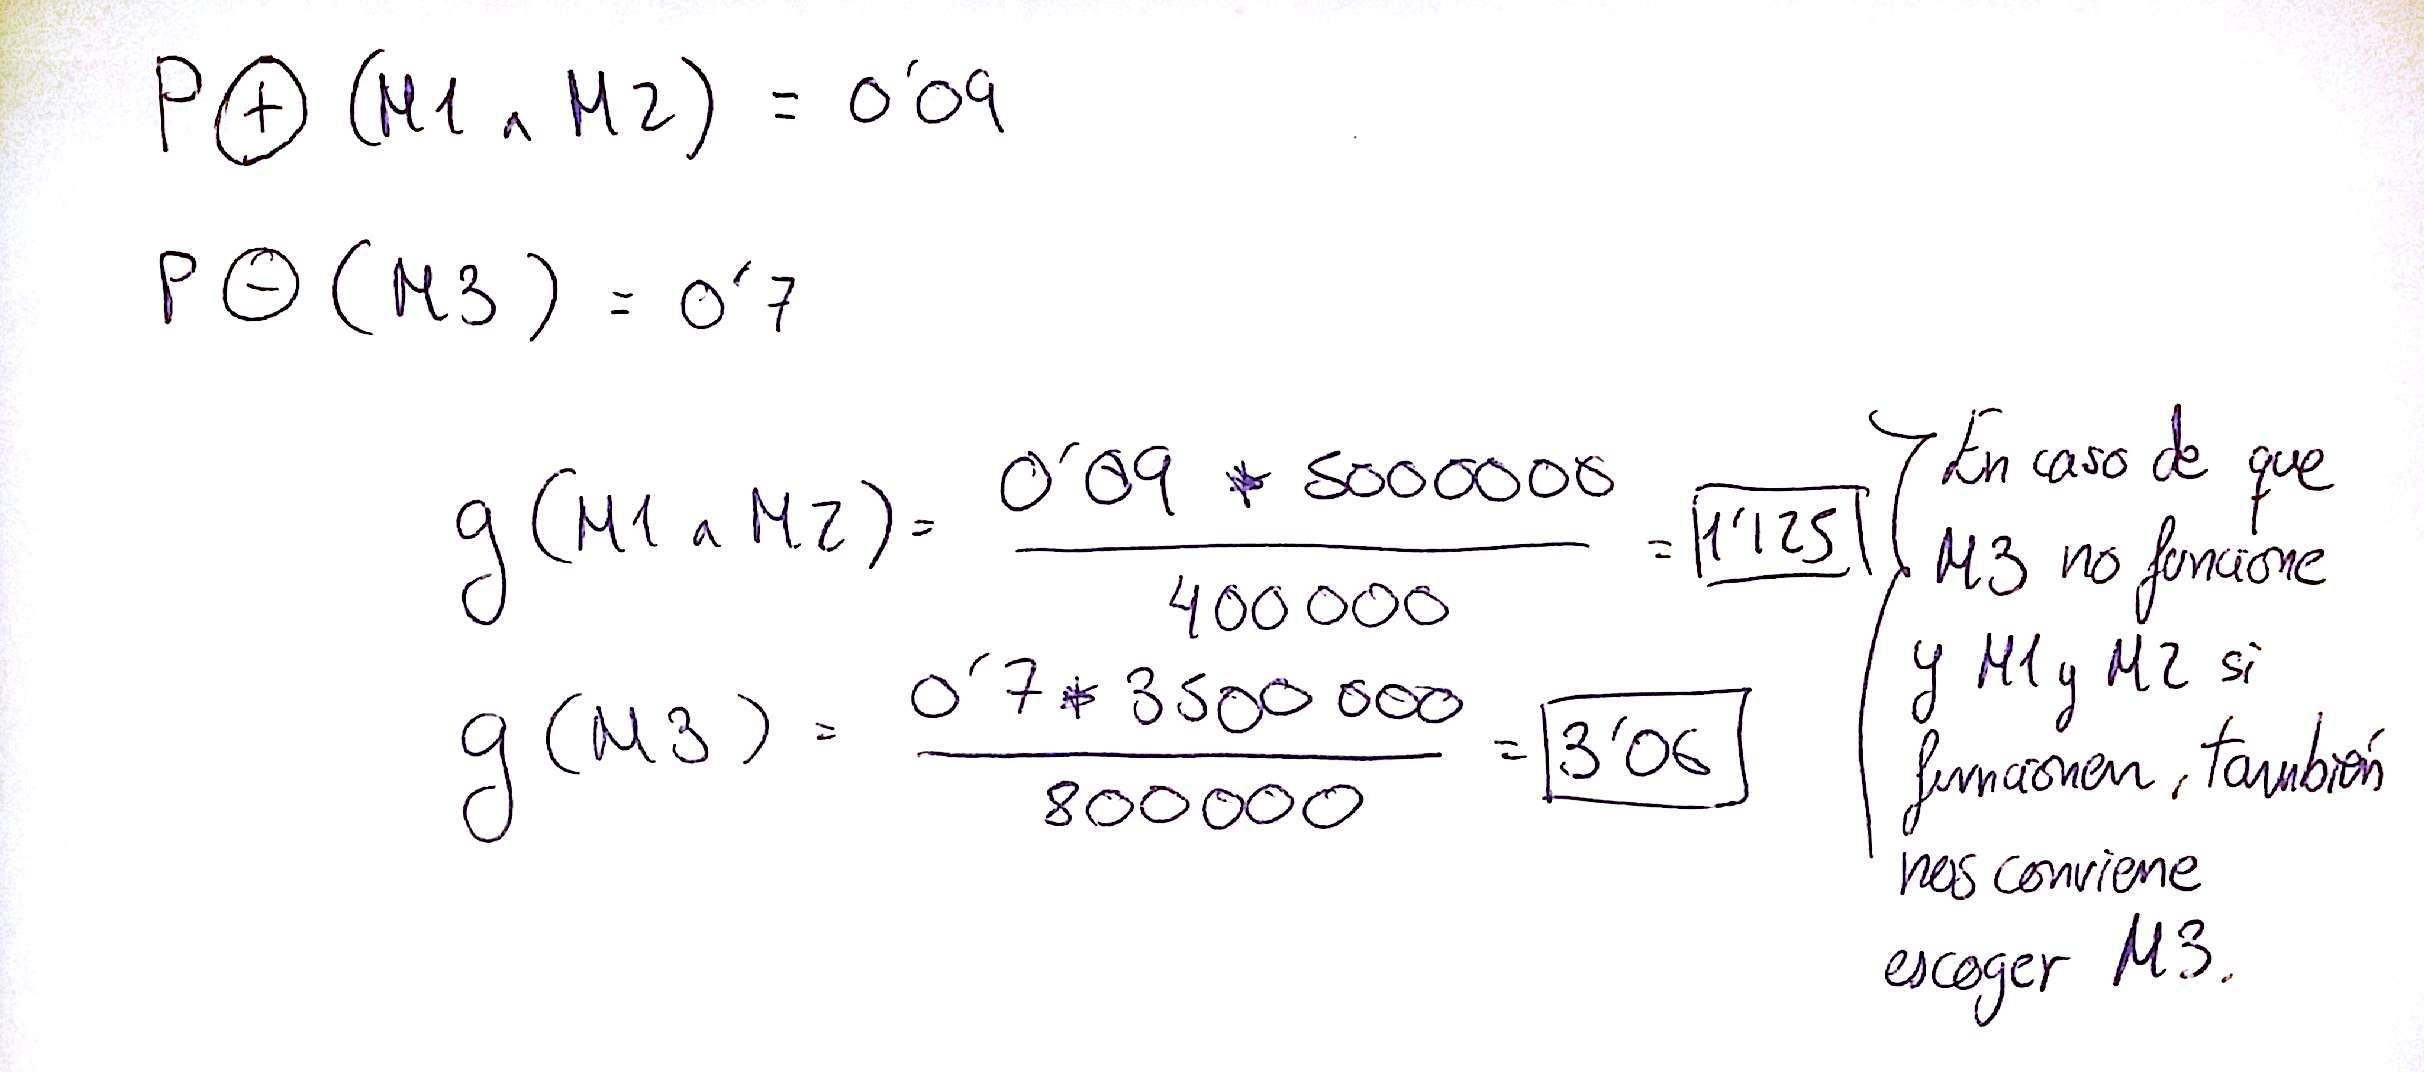
\includegraphics[scale=0.19]{imagenes/ej52} 
\end{figure}

\begin{figure}[H]
	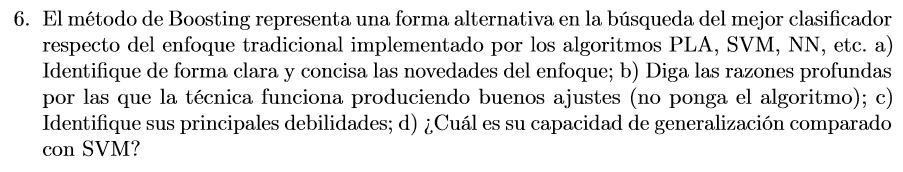
\includegraphics[scale=0.65]{imagenes/6} 
\end{figure}


\textbf{APARTADO A:}\\ La principal novedad ofrecida por dicho enfoque es que pretende conseguir un clasificador robusto (un buen clasificador) a partir de clasificadores debiles (malos, pero levemente mejores que los clasificadores aleatorios). Tambien es una novedad el hecho de que Boosting trabaja sobre el propio conjunto entero de entrada, no realiza particiones sobre el dataset para efectuar la clasificación.
El algoritmo no se basa unicamente en la etiqueta de los datos para clasificarlos, sino en la distribución de probabilidad que tiene cada dato asociada para determinar la posibilidad de ser de una clase o de otra.\\

\textbf{APARTADO B:}\\ El concepto es sencillo: generamos malos clasificadores y juntamos sus resultados para obtener un buen clasificador. A partir de esta idea creo que es fácil pensar en que, lo que no tiene un clasificador, lo puede tener el otro y, a la hora de juntarlos, es posible conseguir un buen resultado debido a esa complementación entre modelos. Además, con el fin de generar distintos modelos de manera que cumplan esa complementacion mencionada entre modelos, los pesos asociados a los datos son manipulados en las sucesivas iteraciones, dando mayor prioridad a los elementos mal clasificados para que en las siguientes predicciones tengan mayor probabilidad de ser bien clasificados.\\

\textbf{APARTADO C:}\\ El mayor inconveniente para el método Boosting es el mal comportamiento ofrecido a la hora de soportar el ruido aleatorio en la clasificación, el cual esta presente en la mayoría (si no en todos) de los problemas de la vida real y por ello hace que su uso sea puesto en duda a la hora de la verdad.\\
Fuente:\cite{ref1}

\textbf{APARTADO D:}\\


\begin{figure}[H]
	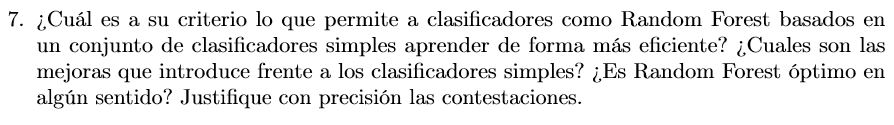
\includegraphics[scale=0.65]{imagenes/7} 
\end{figure}

\textbf{APARTADO A:}\\
Pienso que el factor que mayormente contribuye a la eficiencia de Random Forests es el hecho de que utiliza una cantidad m de atributos (predictores) igual a $\sqrt{p}$, siendo p el número de atributos en la técnica de Bagging. Debido a esto, es decir, construyendo árboles que tan sólo usan m variables seleccionadas de forma aleatoria del conjunto de p predictores, introduce una cierta aleatoriedad que lleva a la disminución de la varianza.\\
Desde el punto de vista de la carga soportada por el sistema utilizado a la hora de aprender, Random Forests genera mas árboles pero de menor tamaño (menor numero de variables), lo que hace que el hecho de aprender sea mucho mas sencillo que aprender con un solo árbol de muchas más variables.\\

\textbf{APARTADO B:}\\
En bagging está presente la existencia de variables correladas debido a que todos los árboles construidos por esta técnica serán parecidos, en consecuencia la varianza no desciende lo deseado.
Random Forests aporta la solución a este problema, haciendo que los árboles que construye Bagging no estén correlados, de esta manera sí habrá una mayor reducción de la varianza respecto del método de Bagging.\\
También introduce aún una mayor aleatoriedad que Bagging, debido a que escoge el subconjunto de m variables del conjunto de atributos p y, además, es capaz de dar estimaciones acerca de las variables con mayor importancia en la clasificación.\\

\textbf{APARTADO C:}\\
Pienso que no es un método de aprendizaje óptimo, puesto que está comprobado que con algunos grupos de datos Random Forests realiza sobreajuste sobre tareas de clasificación/regresión ruidosas.
Fuente:\cite{ref2}

Otro de los posibles fallos es que, el hecho de que tan solo se escoge un subconjunto \textbf{m} de los \textbf{p} atributos disponibles para aprender los modelos, me induce a pensar en que quizás el aprendizaje no es tan completo como el realizado por Bagging, el cual sí utiliza los p predictores disponibles.


\newpage
%------------------------------------------------

\bibliography{citas} %archivo citas.bib que contiene las entradas 
\bibliographystyle{plain} % hay varias formas de citar



\end{document}
